% ---------------------------------------------------
% ----- Chapters of the template
% ----- for Bachelor-, Master thesis and class papers
% ---------------------------------------------------
%  Created by C. Müller-Birn on 2012-08-17, CC-BY-SA 3.0.
%  Freie Universität Berlin, Institute of Computer Science, Human Centered Computing. 
%
\chapter{User research and analysis}
\label{chap:research}


Over ten years after the publication of Tomer Sharon's book ''It's our Research'', the list of quotes in the introduction about user research in software companies still feels as relevant as ever.
\\
''Yeah, but this study will delay our launch date.'', ''Yeah, but we can not learn much from only five participants.'', ''Yeah, but research sounds so academic.'' \cite[p. 4]{Sharon:2012mk} are only some of the statements that according to Sharon are often heard in software companies in discussions about User Experience (\Gls{ux}) research.
\\
The pressure from stakeholders often leads to quick implementation of features and workflows without figuring out the user's needs.
This seems faster in the beginning, but can badly impact the user's acceptance of the product due to cumbersome and slow workflows,
in the worst case it leads to the refusal of the whole product.

To counteract this, it is crucial to conduct user research methods and evaluate the user's needs.
This fact is considered in the development of the UI Editor.
A starting point for qualitative user research is to define the goals through the help of the SMART criteria, which provide guidelines and formulated goals during research.
For the project, the SMART criteria were defined like this:
\label{fig:smart}
\begin{itemize}
  \item \textbf{specific} - improve the workflow of users modifying dynamic resources for \Gls{experience}
  \item \textbf{measurable} - interviews after testing period concerning working speed, confidence and joy when editing resources, automated user tracking
  \item \textbf{achievable} - research and implementation will mostly be conducted by me, with input from CTO \& product owner, connections to external users through customer service team
  \item \textbf{relevant} - new software platform which reacts quicker, provides more safety regarding errors and is scalable and extensible in the future.
  \item \textbf{time-bound} - the new software should have a feature set enabling productive work, replace the old \textit{Storefront Editor} and be usable by company internal users until the end of 2022
\end{itemize}
Remembering these points was helpful when the focus on the actual goals was unclear.
\\\\
In addition, Becker (\cite[pp. 37-41]{LearnHCI:2020ys}) states that there are ``three major factors that an HCI designer should consider''.
These three factors were seldom mentioned in publications but are helpful guidelines.
\begin{description}
  \item[Usability Factor] describes the spectrum from ''usable'' to ''unusable'' software. This is determined by the implemented software design features and how they support the user achieve their tasks in the environment provided.
  \item[Accessibility Factor] is high when as many users from different backgrounds can use the software in different environments. 
  It includes access for people with and without disabilities as well as low entry hurdles for new users.
  At first glance this factor does not look as important as the other two, especially for specialized applications, but it should not be left out when designing and implementing software.
  \item[Time-On-Task Factor] refers to ''[...] solutions that use up the appropriate of time to solve a problem.'' \Cite[p. 40]{LearnHCI:2020ys}. Obviously, to save users time, a fast system is required.
But it is inevitable that network delay computation tasks all require some time, and users understand that fact. More important is reducing the perceived lag of interactions and give users feedback if a task takes longer to complete.
\end{description}

\section{Identifying and categorizing users and user groups}
\label{sec:user-groups}
In order to effectively design and implement the UI Editor, it is crucial to understand the needs and preferences of the various users and user groups who will be using the tool.
The first step in the process was to identify and categorize them.
Then, detailed information is gained through the observations and interviews (\ref{subsec:modobs} and \ref{subsec:interview}) and finally concrete Personas for the different user groups are built (\ref{subsec:personas}).
\\
It was easy to collect a list of potential users for the new UI Editor because Sprylab already had users working with the ecosystem and the predecessor of the editor.
A larger group of different users or external customers would require more effort to perform this step though.
\\
The next step was grouping them to understand the characteristics and needs of each user group.
Having this overview made it easier to tailor the UI Editor to their specific requirements so it can be used effectively by all users\footnote{``All users'' refers to users that are expected to work with the tool. There is an expected technical and domain specific base knowledge that the UI Editor won't cover in its initial form}.
Also, when choosing who to use as research subjects this list can help to get broad coverage of users with different needs and abilities.
\\
The information about the users leads to the following common factors:
\begin{description}
  \item[Quantitative usage -] Some users rely on the tools for most of their work, others a few times a year.
  \item[Common tasks -] I roughly categorized the common tasks into three groups:
  \begin{description}[nosep]
    \item[Heavy configuration -] Build new apps and websites from scratch, making a wide range of modifications and structural changes.
    \item[Moderate configuration -] Copying resources from templates and adapt them for new brands, which includes changing colors and logos, adapting texts or switching authentication flows.
    \item[Small changes -] Exchange ads, translations or logos, which affects a small set of files.
  \end{description}
  \item[Expertise] -
  \begin{description}[nosep]
    \item[Technical -] Depending on the area of education and work experience in web development, knowledge about web standards and often also intuition differs between users.
    \item[Domain- and Platform Specific -] Special vocabulary, functionality of Purple Experience and other systems as well as configuration tricks that users learn with time.
  \end{description}
\end{description}

% ... more
\section{Qualitative user research}

The existing user base, most of them at Sprylab, simplified access to participants for qualitative user research methods.
Using one or multiple ways of triangulation \cite[p. 264]{Interactiondesign:2019ys} can strengthen the significance of the research outcome. Limitations of method or source can be removed by variation of those, resulting in a less distorted picture.
Therefore, methodical triangulation\footnote{Using multiple data gathering techniques} as well as triangulation of data\footnote{Collecting data from different people and different sources} seemed well suited.
Moderated observations combined with interviews proved to be a good fit for this case study, as they are interaction driven and the observer can react directly on behaviors / emerging topics and steer the process.
This stands in contrast to more passive methods like passive observations or user recording and tracking analysis, where the outcome only depends on the
prepared question / task and the user's behavior and which can not adapt to changed circumstances etc. during the application.
\\\\
The chosen structure for the observations and interviews looks like this:

\begin{description}
  \item [Introduction (ca. 5min)] used to explain the circumstances and the goal of the session, the method, which data will be collected and how they will be evaluated afterwards.
  \item [Moderated Observation (10-15min)] let the observed perform specific tasks in a prepared environment
  \item [Semi-structured Interview (ca. 15min)] ask open and closed questions and discuss observation situation
\end{description}
Interviews came after observations to allow discussing issues encountered during the moderated observation and to gain deeper insight into the workflow and potential problems.
\\
To verify the methodical approach and whether the concrete questions fit the process and can yield desired information, it was important to pretest the whole process with a small group before scheduling the other meetings. One of Sprylab's working students agreed to be a test candidate and we verified the prepared tasks and questions I planned.
Pretesting the methods and specific questions before conducting them on a broader audience helped to sharpen them by identifying ambiguous, repetitive or already known facts.
For the tasks of the moderated observation the test gave feedback on the difficulty, time the sessions would probably take on average, which tasks needed clearer formulations and which were already sufficient.
\\
The user research was conducted with six persons, including a core Purple Experience developer, two working students from our project department, one developer from a different department who had worked with the software some time prior, one Customer Support Manager from Sprylab and one external user from a publisher.
\\
An interesting concept relevant for the choice if subjects from \cite[p. 41]{AboutFace:2014ys} is the Subject Matter Expert (SME), who represents ``authorities on the domain on which the product will operate.'' \cite[p. 41]{AboutFace:2014ys}. The SME is important for the process to give input on technical details and patterns other less involved users might not know. For this case study, the Purple Experience developer represents the SME for the underlying platform the UI Editor is built for.

\subsection{Moderated observation}
\label{subsec:modobs}
For the moderated observation a list of six tasks was prepared. Two of them were optional depending on the time left and how familiar the user felt with dynamic resources.
The same first tasks could be given to every interviewee regardless of their level of knowledge, the optional tasks if there was still enough time.
Also, it was important that the tasks did not build on each other to prevent the observed person getting stuck because of an earlier mistake.
Instead, seeing a variety of tasks getting performed gave more insights than one task being executed without errors. 
Therefore, an example app was created on Sprylab's staging system, so it was easy to prepare and also reset after each observation session.
\\\\
The six tasks were:
\begin{enumerate}[itemsep=0mm]
  \item Change app menu entry "Newsstand" to "Home" on all platforms (Web, Android and iOS).
  \item Change the advertisement banner target on top of the home page to https://google.com. 
  \item Change the text "Latest Issues" on the home page to "Read new Issues".
  \item Change color of "Read new Issues" and "Latest Articles" headers on the home page to the app's primary color..
  \item \textit{(Optional)} Add a dropdown on the home page between "Read new Issues" and "Latest Articles"
    \subitem It should show all publications connected to the app
    \subitem It should set a URL parameter ``publication'' to the id when selected
    \subitem Define the reset message as ``All publications''
  \item \textit{(Optional)} Configure the filter of the ``Latest Articles'' list to only show articles from that publication
\end{enumerate}

These tasks were constructed in a way that errors could occur and were expected, which allowed to see how users try to figure the cause of the problem out and how to fix it.
As expected these cases then also occurred, for example the first task was often done for only one of the three platforms, the ``Latest Issues'' text (task 3) was not found in the translation files or the color change was applied to more elements than desired (task 4).

The optional tasks were presented to four people, of which three solved at least one task successfully, only the core developer solved all six tasks completely.
With the consent of the interviewees I recorded their screens during the observation to rewatch specific actions or flows if required.

\subsection{Interview}
\label{subsec:interview}
For the interview, a semi-structured interview was chosen as the appropriate tool.
With a list of open and closed questions the interviewer can ensure that important topics are covered.
Furthermore, it allows flexibility to delve deeper into specific issues and ideas if needed.
\\
The prepared questions consisted of closed ones, like how often they interact with the tools, how confident they feel implementing changes or fixing errors, and open questions like to describe step by step what the most recent task was they performed with dynamic resources, how they were onboarded etc.
If notable points occurred during the observation, these were addressed now either directly or in form of an open question like ``If you imagine a UI builder with no technical limits, how would it look like, which features would you expect and what workflows are most important to you?''.
\\
The semi-structured interviews proved to be valuable in gaining insight into the experiences and needs of the users. They made it possible to gather lots of new information and show how different features were massively valued differently by the users. Two interviewees even provided written lists of their ideas and suggestions afterwards.
\\\\
Here are some examples of the outcomes:
\begin{itemize}[itemsep=0mm]
  \item The way users validate their changes differs widely; some use a preview window in the old editor, some merge changes into the resources and view it on the website or inspect the app's JavaScript context, some prefer separate windows, some embedded frames to see code and preview at the same time.
  \item Rearranging or adapting the layout of the tools / editor to match the current screen and browser window size is important, e.g. hide unnecessary panes if not used, make the window the user currently works in larger to see more content at once.
  \item Editing multiple files at once (in the old editor one could only edit one file at a time, had to close the current and open the next one).
  \item Collaborative working: Seeing the current state of the resources, e.g. if a live or preview resource is processing, if other users are working in the same app parallel, and having git-like line-by-line diffs of the changes made.
\end{itemize}
\bigskip
Some outcomes from the user interviews will be further discussed in chapter \ref*{chap:impl}.

\section{Quantitative user research}

At the initial stages of research, the use of questionnaires was considered as a method of gathering information from existing and potential users.
However, as the outcome of the qualitative research was already productive, it proved difficult to design a questionnaire that would provide additional information while adhering to common design rules for questionnaires in terms of length, number and type of questions.
Prototype questionnaires were created using Microsoft Forms, but they were too long, difficult to understand, or not relevant to the development of prototypes.
Therefore, it was decided to rely solely on qualitative research results for prototyping and feedback, along with some automatic tracking implementation (see \ref{sec:analytics}).
\\
\section{User research outcomes}

After each observation and interview, which were additionally recorded, the interviewer noted facts about the subject and the session in a prepared template.
The mandatory fields consisted of basic information like the role of the user, frequency and typical tasks with the resources.
Additionally, important situations from the observation, a description of the workflows, input from the interview and the linked recordings were noted.

A shortened and anonymized version of the notes can be found in the Appendix \ref{app:interviews}.
Derived from these notes, combined with the technical requirements, the following subset of essential features emerged:

\begin{description}[nosep]
  \item[App Selection] \leavevmode
  \begin{itemize}
    \item Having quick access to recently opened apps, search by App name, App ID and Publisher Name.
  \end{itemize}
  \item[App Editing] \leavevmode
  \begin{itemize}[itemsep=0mm]
    \item Automatic downloading and packing of the dynamic resource ZIPs so manual pack/unpack operations are not required by the users.
    \item Support for syntax highlighting and autocomplete for common files.
    \item Fast load times or the possibility to have multiple files open simultaneously.
  \end{itemize}
  \item[App Preview]\leavevmode
   \begin{itemize}[itemsep=0mm]
    \item See a frame on the side / in extra window showing the latest changes instantly, load "real" data from the API.
    \item Ability to load current state of config and assets inside an app connected for debugging.
  \end{itemize}
  \item[Dynamic Resource Change Management] \leavevmode
  \begin{itemize}[itemsep=0mm]
    \item See which files were changed since last upload.
    \item Reset single files to an earlier version.
    \item Have version control features like "commit messages" and version diffs.
    \item See who uploaded new changes and if changes are being processed.
  \end{itemize}
\end{description}


\section{Process and visualize the research outcomes}

To gain as much value from the raw research data it is crucial to find methods to process and visualize the outcomes.
A common approach at companies is to write "tickets" in their ticket system of choice, in case of Sprylab Jira (\url{https://www.atlassian.com/de/software/jira}).
From my experience, Jira and co. prove valuable to track progress during development.
It is not suitable for discovery and prioritization of features at the beginning because lists of tickets with different priority levels and different sorting do not give a good overview over effort and benefit of each feature.
Thus, based on the notes from observations and interviews two alternative ways were tried to figure out different features and how they can be prioritized.

\subsection{2x2 Opportunity Matrix}

Fig. \ref{fig:opportunitymatrix} shows a two-dimensional visualization of a subset of proposed features.
It proved helpful when prioritizing tasks with other stakeholders,
as it shows the approximated cost of implementation as well as the value the feature can have for users.
Costs include possible financial costs as well as required time and amount of resources needed to implement the feature.

It is a slightly modified adaption from \cite[p. 181]{LearnHCI:2020ys}, replaced the term ``idea originality'' on the x-axis with ``Value''.
The benefit of visualizing multiple possible features is to see at one glance the relation between value for users but also cost of implementation in a more clear way than lists of tickets with different priorities would provide.

\begin{figure}[h!]
	\centering
  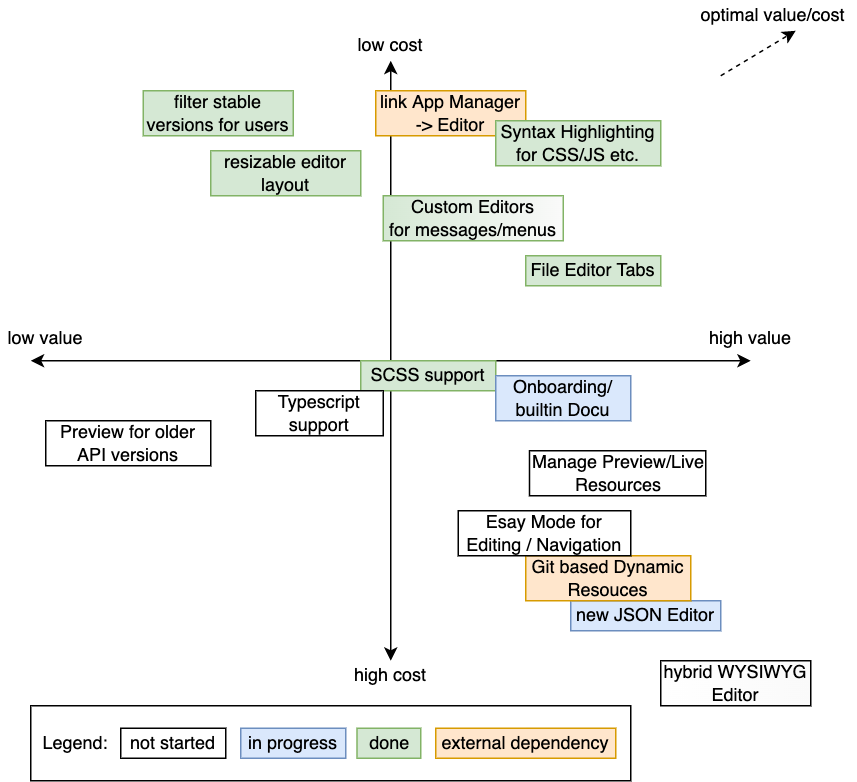
\includegraphics[width=\textwidth]{pics/feature_cost_matrix.drawio.png}
	\caption{2x2 Opportunity Matrix during the early phases of development (adapted from \cite[p. 181]{LearnHCI:2020ys})}
	\label{fig:opportunitymatrix}
\end{figure}


\subsection{Building Personas}
\label{subsec:personas}

Personas are descriptions of fictional users of the product, incorporating assumptions and optionally data for a user group.
They aim to give developers and designers more context and depict real potential users, which makes it easier for a developer to empathize with the user.
For this case study three Role-based Personas were derived from \ref{sec:user-groups} and the outcomes of the interviews, based on the description of Personas in \cite[pp. 403-405]{Interactiondesign:2019ys}. They can be found in Appendix \ref{app:personas} and represent the users with different levels of expertise already identified in \ref{sec:user-groups}.